\defverbatim[colored]\lstI{
\begin{lstlisting}[language=C++,basicstyle=\ttfamily,keywordstyle=\color{red}]
#include <linux/bpf.h>

int prog(struct xdp_md *ctx){
    return XDP_DROP;  // descarta todos pacotes
}
\end{lstlisting}
}


% Dados referentes ao número de usuários da internet
\section{Contextualização}
\begin{frame}{}
	\begin{figure}
		%\caption{Número de usuários ativos em 2019}
		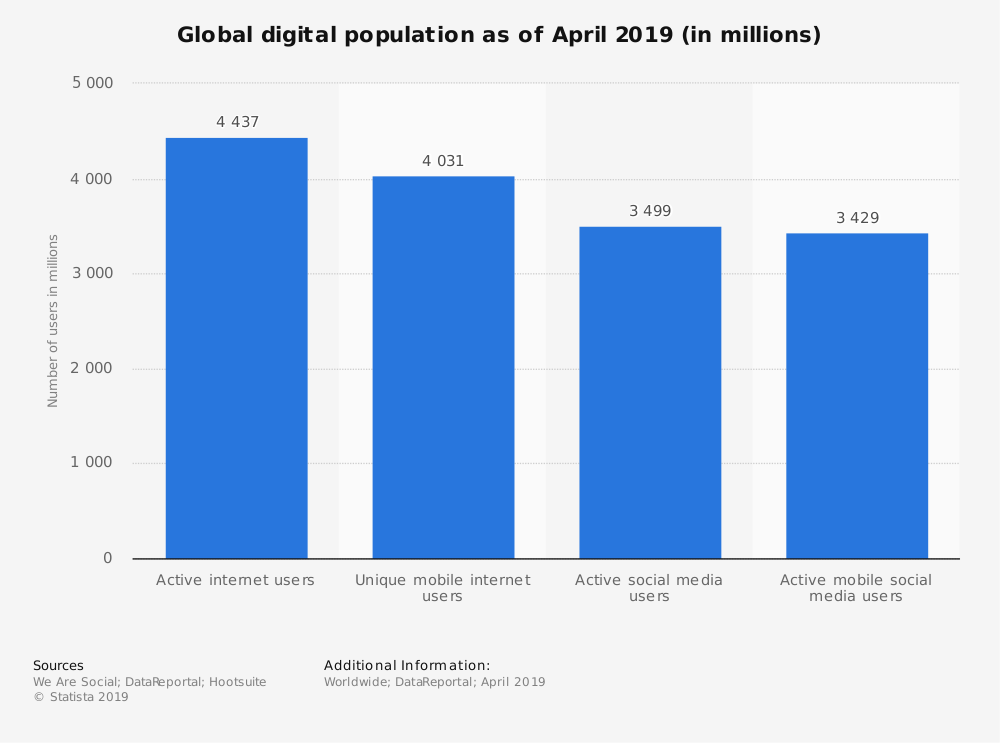
\includegraphics[width = 0.85\linewidth]{img/proj_tcc/statistic_id617136_worldwide-digital-population-as-of-april-2019.png}\\
		\tiny Fonte: We are Social; Data Reportal; Hootsuite
	\end{figure}
\end{frame}

% Modelos de negócios dependem cada vez mais da rede e demandam conexões de menor latência e maior segurança
\begin{frame}{}
	\begin{figure}
        \centering
        \begin{minipage}{.5\textwidth}
          \centering
          
\includegraphics[width=.5\linewidth]{img/proj_tcc/uber.jpg}
          \captionof{figure}{Transporte}
          \label{figure:facebook}
        \end{minipage}%
        \begin{minipage}{.5\textwidth}
          \centering
          \vspace{15pt}  % Just for alignment
          
\includegraphics[width=.7\linewidth]{img/proj_tcc/netflix.png}
          \captionof{figure}{Filmes}
          \label{figure:cloudflare}
        \end{minipage}
    \end{figure}	
    \begin{figure}
        \centering
        \begin{minipage}{.5\textwidth}
          \centering
          
\includegraphics[width=.5\linewidth]{img/proj_tcc/whatsapp.png}
          \captionof{figure}{Comunicação}
          \label{figure:facebook}
        \end{minipage}%
        \begin{minipage}{.5\textwidth}
          \centering
          %\vspace{10pt}  % Just for alignment
          
\includegraphics[width=.5\linewidth]{img/proj_tcc/bitcoin.png}
          \captionof{figure}{Moeda}
          \label{figure:cloudflare}
        \end{minipage}
    \end{figure}
\end{frame}

% No caso de redes IoT, onde muitos dispositivos trocam mensagens (que muitas vezes carregam informações sensíveis) entre si e com a internet, essa realidade é ainda mais complicada.
\begin{frame}{}
	\begin{figure}
		\caption{}
		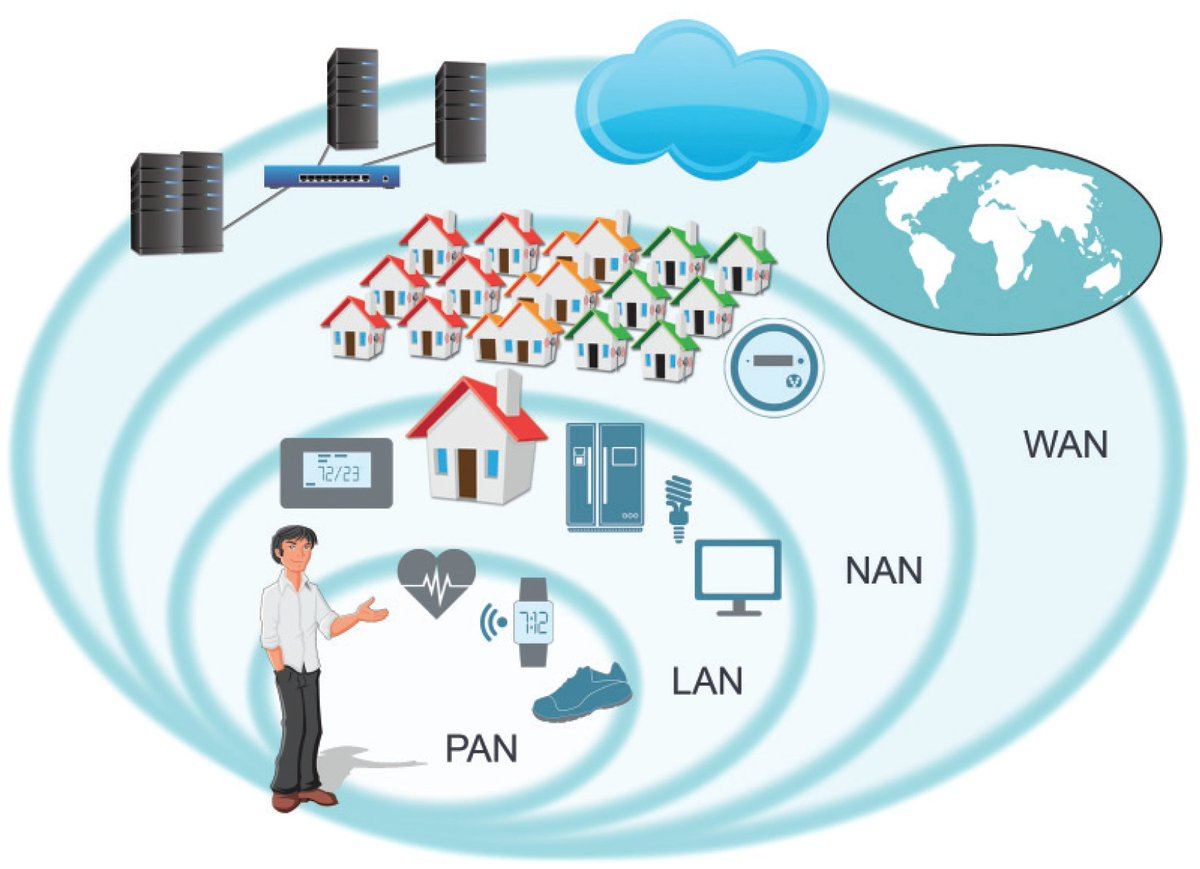
\includegraphics[width = 0.8\linewidth]{img/proj_tcc/iot_network.jpg}\\
		\tiny Fonte: VectoMobile
	\end{figure}
\end{frame}

% Surge a necessidade de dinamizar a rede inserindo programabilidade e a tornando flexível e mais segura.
\begin{frame}{Programabilidade de redes}
	\begin{itemize}
	    \item Dinamicidade e Flexibilidade
	    \item Gerência facilitada
		\item Segurança (remediação e predição)
		\end{itemize} 
\end{frame}


% eBPF + imagem do facebook e Cloudfare
\section{eBPF (extended Berkeley Packet Filter)}
\begin{frame}{eBPF - extended Berkeley Packet Filter}
\begin{itemize}
		\item Máquina virtual no kernel (\textit{segurança}).
		\item Interface dinâmica entre \textit{user space} e \textit{kernel space}.
		\item Alternativa flexível aos módulos atuais do kernel.
	\end{itemize} 
\begin{figure}
\centering
\begin{minipage}{.5\textwidth}
  \centering
  
\includegraphics[width=.4\linewidth]{img/proj_tcc/facebook-logo.png}
  \captionof{figure}{Balanceador de carga}
  \label{figure:facebook}
\end{minipage}%
\begin{minipage}{.5\textwidth}
  \centering
  \vspace{28pt}  % Just for alignment
  
\includegraphics[width=.6\linewidth]{img/proj_tcc/cloudflare.png}
  \captionof{figure}{Mitigação de ataques}
  \label{figure:cloudflare}
\end{minipage}
\end{figure}	
\end{frame}

% imagem com arquitetura da vm e workflow (passos e maps)
\begin{frame}{eBPF - extended Berkeley Packet Filter}
    \begin{figure}
        \centering
        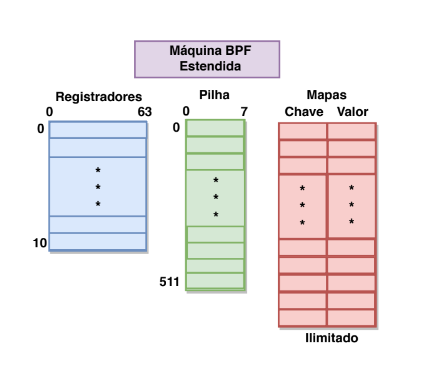
\includegraphics[width=.55\linewidth]{img/proj_tcc/maquina-ebpf.png}
        \label{figure:facebook}
    \end{figure}
    \begin{figure}
      \centering
      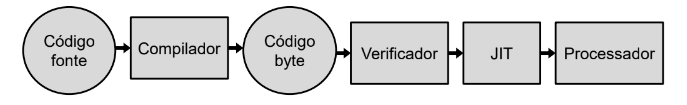
\includegraphics[width=.8\linewidth]{img/proj_tcc/workflow.png}
      \label{figure:cloudflare}
    \end{figure}
\end{frame}

% empregos do eBPF
\begin{frame}{eBPF - extended Berkeley Packet Filter}
    \begin{itemize}
        \item kprobes (uprobes, kretprobes, uretprobes)
        \item socket filter
        
        ...
        
        \item XDP (\textit{eXpress Data Path})
    \end{itemize}
\end{frame}

% eBPF e XDP. Figura da pilha de rede do kernel e explicação do funcionamento
\begin{frame}{eBPF \& XDP (\textit{eXpress Data Path})}
	\begin{figure}
		\caption{}
		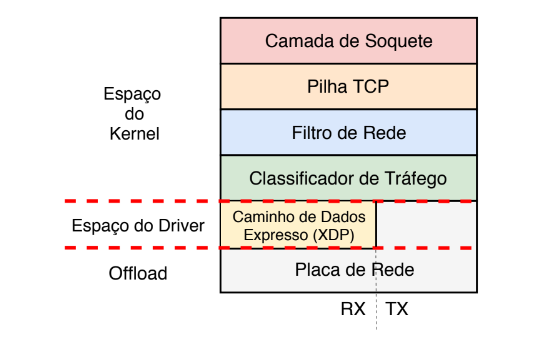
\includegraphics[width = 0.65\linewidth]{img/proj_tcc/kernel-network-stack.png}\\
		\tiny Fonte: HootSuite, Abril de 2019
	\end{figure}
\end{frame}

% código simples que realiza o descarte de todos os pacotes

\begin{frame}{eBPF \& XDP (\textit{eXpress Data Path})}
\lstI
\end{frame}

% Segurança e monitoramento em IoT para mitigação e identificação de ataques
\begin{frame}{IoT (\textit{Internet of Things})}
    \begin{enumerate}
        \item Monitoramento
        \item Análise estatísica (Wi-Fi, LoraWan, NFC, etc.)
        \item Intervenção dinâmica (eBPF)
    \end{enumerate}
\end{frame}

% Básica, Exploratória, Bibliográfica e Experimental
\section{Pesquisa}

\begin{frame}{Objetivo}
    \begin{enumerate}
        \item Aprofundamento dos conhecimentos referentes ao arcabouço eBPF e pleno entendimento das oportunidades.
        
        \vspace{30pt}
        
        \item Experimentação em projetos de infraestruturas de IoT com incorporação do eBPF.
    \end{enumerate}
\end{frame}

\begin{frame}{Metodologia}
\begin{itemize}
		\item Básica
		\item Exploratória
		\item Bibliográfica
		\item Experimental
	\end{itemize} 
\end{frame}

\begin{frame}{Cronograma}
\begin{itemize}
		\item 6 meses de pesquisa.
		\item Laboratório de computação distibuída (LCD).
	\end{itemize}

	\begin{table}[]
        \centering
        \begin{tabular}{|l|c|c|c|c|c|c|}
        \hline
        \multicolumn{1}{|c|}{Atividade / Meses} & Jul & \multicolumn{1}{l|}{Ago} & \multicolumn{1}{l|}{Set} & \multicolumn{1}{l|}{Out} & \multicolumn{1}{l|}{Nov} & \multicolumn{1}{l|}{Dez} \\ \hline
        Pesquisa Bibliográfica                  & X     &                             &                               &                              &                               &                               \\ \hline
        \textit{Estruturação do projeto}        &       & X                           &                               &                              &                               &                               \\ \hline
        \textit{Planejamento da experimentação} &       & X                           &                               &                              &                               &                               \\ \hline
        \textit{Experimentação}                 &       &                             & X                             & X                            &                               &                               \\ \hline
        Tratamento de resultados                &       &                             &                               & X                            &                               &                               \\ \hline
        Relatório final                         &       &                             &                               & X                            & X                             &                               \\ \hline
        Revisão / correção do texto             &       &                             &                               &                              &                               & X                             \\ \hline
        \end{tabular}
        \label{table: Cronograma de pesquisa}
    \end{table}
\end{frame}

% Exploração e compreensão dos limites da tecnologia, bem como a projeção de uma infraestrutura que provê uma melhora na latência e/ou segurança
\begin{frame}{Resultados Esperados}
\begin{itemize}
		\item Autonomia para implementações envolvendo eBPF.
		
		\vspace{30pt}
		
		\item Protocolos que melhor usufruem do eBPF para melhoria em \textbf{latência} e \textbf{segurança}.
	\end{itemize} 
\end{frame}
